\chapter{Multi-central healthcare ecosystems}

\label{Bookchapter}

\begin{abstract}
\dropcap{W}ith recent developments in medical imaging facilities, extensive medical imaging data is produced every day. This increasing amount of data provides an opportunity for researchers to develop data-driven methods and deliver better healthcare. However, data-driven models require a large amount of data to be adequately trained. Furthermore, there is always a limited amount of data available in each data center. Hence, deep learning models trained on local data centers might not reach their total performance capacity.
One solution could be to accumulate all data from different centers into one center. However, data privacy regulations do not allow medical institutions easily combine their data and this becomes increasingly difficult when institutions from multiple countries are involved. Another solution is to use privacy-preserving algorithms, which can make use of all the data available in multiple centers while keeping the sensitive data private. Federated learning (FL) is such a mechanism that enables deploying large-scale machine learning models trained on different data centers without sharing sensitive data. In FL, instead of transferring data, a general model is trained on local datasets and transferred between data centers. FL has been identified as a promising field of research, with extensive possible uses in medical research and practice. This paper introduces FL, with a comprehensive look into its concepts and recent research trends in medical imaging.


\end{abstract}

\blfootnote{This chapter is partly based on \faFileTextO~\emph{E. Darzidehkalani et al. Federated learning in
medical imaging
Part (I): towards
multi-central healthcare
ecosystems, and E. Darzidehkalani. Federated learning in
medical imaging
Part (II): methods, challenges and considerations}.
}


\newpage

% \dropcap{T}his is a introductory page.



% keywords can be removed
% \keywords{Federated learning \and Privacy-preserving machine learning \and  Medical imaging}


\section{Introduction}

\dropcap{D}eep learning has shown great promise in the field of radiology. It has been used extensively in various medical imaging domains and has already helped clinicians and radiologists in numerous ways. The area of radiology has dramatically benefited from deep learning research. It has been shown that deep learning can improve the existing models of tumor detection, from early processing stages such as image enhancement in Magnetic Resonance Imaging (MRI) and Computed Tomography (CT), noise reduction, lesion detection, and segmentation, disease monitoring. All of these areas have shown great promise for the use of artificial intelligence in clinical settings. 

 Deep neural networks are made up of many layers with billions of parameters, and they train to learn a complex, high-dimensional mapping from raw input data to desired labels.\cite{erfani2016high} The main issue with training deep neural networks in real-world medical practice is that a massive amount of diverse data is needed. A neural network trained on a single dataset from a single institute may be easily overfitted, resulting in a strong bias towards that institute and poor generalization. Furthermore, latent patterns in one client's imaging data may influence the performance of a neural network in ways that have nothing to do with the actual biological way in the image. For example, datasets containing only one modality or images registered on a specific atlas may bias deep learning models towards that modality or atlas, capturing irrelevant data as significant predictors. The quality of data of a single institution depends on a variety of factors such as the number of patients, type or number of imaging machines available,  and the number of experts available at that institution. Not all healthcare facilities have vast amounts of diverse imaging data, and deep learning models are thus usually trained on limited datasets. This makes clinical decision-making burdensome given the low number of cases, which happens more often in rare diseases. \newline One potential solution to this data shortage is to obtain imaging datasets from different clients. This method has the potential to increase both the amount and diversity of data collected. The most frequent method for establishing such a  collaboration is to centralize vast and diverse datasets from multiple institutions and train a deep neural network on an accumulated dataset situated in a central hub, as can be seen in Figure \ref{fig:CDS}. However, this technique is fraught with difficulties; strict national or regional privacy rules, such as GDPR in Europe or HIPAA in the United States, preclude institutions from easily sharing their patients' data. Other impediments may arise due to the multiple stakeholders, including hospitals, patients, researchers, medical physicians, and industrial corporations, each pursuing their interests. The significant amount of time and effort (and hence money) that an institution spends to collect and clean data makes it hesitant to share it with other institutions.
% Another application is for patients with a rare disease. It is often impossible for a single institution or even multiple institutions to reach a consensus about diagnosis, treatment, ...etc of a rare disease given a low number of cases. 

\begin{figure}[h!]
 \centering
  
\includegraphics[scale=0.31]{Centrlizied algorithm.jpg}
  \caption{Centralized data sharing (CDS)}
  \label{fig:CDS}
\end{figure}

Recent advancements in privacy-preserving AI algorithms play an essential role in solving this. They enable researchers and institutions to train their networks on diverse imaging data from multiple institutions while ensuring that data will be kept locally, thus avoiding many issues concerned with building and maintaining an extensive central database. A general methodology in deep learning is decentralized or distributed learning. Distributed learning can be defined as a group of algorithms in which multiple clients do part of the computation or data storage tasks. The data distribution allows numerous clients to participate in the learning process and enables higher performance with a larger input data size. It generally involves multiple nodes and clients doing partial computation, each on then own local database. Distributed learning is done for a variety of reasons, including performance boost and large-scale computation. Federated learning is a version of distributed learning tailored for tasks where data privacy is essential so that researchers can preserve privacy while performing distributed learning. This feature enables healthcare centers to train deep learning models without compromising the privacy of their local data. 


\section{Federated learning algorithms}
\label{sec:FL algorithms}


A deep learning model is a form of algorithm based on artificial neural networks. It utilizes high volumes of data to extract patterns from them. Artificial neural networks generally consist of millions of parameters called model weights. Training a model is the process of tuning the parameters of the neural network to perform a task ( e.g., detection, classification, or segmentation in the imaging domain). The training process is done by exposing the model to a specific dataset for several rounds. 
More rounds and more extensive training data generally lead to more accurate parameter tuning and better model performance.  Generally, models size depends on their complexity and the number of parameters they have, regardless of how much data they were trained on. Popular deep learning models have a size of no more than around 150 megabytes \cite{canziani2016analysis}.

As a result, complex patterns of enormous imaging datasets can be encoded in models with much smaller sizes. One immediate advantage coming from this feature is in distributed settings. Sharing models in these situations would be much more practical than sharing data. Sharing models are thus subject of interest in distributed settings involving voluminous data, e.g., high-resolution images or multi-slice MRI and CT scans.  \\

Federated learning is a distributed learning method in which multiple participants train (or update) a local model on their data without actually sending data to the central node. A global model is updated according to the updated models received from participants. This way of training allows researchers to ensure the privacy of models and distributes the heavy computing process. FL is also efficient in communication since generally, only model weights will be communicated in this setting. In this regard, it tackles the infrastructural barriers of moving large volumes of data from one institution to another. Various ways to harmonize global and local model updates result in multiple versions of FL. Generally, federated networks require multiple clients who hold the data and perform the local training and a central trusted server, which manages the whole process. \\
% \hl{(Can you elaborate on this. Not every physician/radiologist knows what is model weight and why is it smaller) What gets deleted apart from patients identifier? Do you change the image format? How does this affect image resolution? Can you still PACS system to see the images? How about high resolution mammograms with microcalcifications?.}

\begin{figure}[h!]
 \centering
  
\includegraphics[scale=0.17]{figs/training ga.jpg}
  \caption{Communication between client and server, exchanging the model}
 \label{fig:train1}
\end{figure}


Each client trains a model it gets from the central server on its local data. To get the model, the client sends a request to the cloud server, informing that it's ready to start the local training session. Then the request is processed, and the latest global model is sent back to the client. Next,  the training session starts using the received model and local data. After the local training session is finished,
the model is returned and the center accumulates the received updates. Finally, the global model is updated by the server based on the received model and notifies the client that one training round is successfully completed.  A schema of these steps can be found in the Fig. \ref{fig:train1}.  It is important to note that the model used for training in the hospital has to be the same type as the model being used by the central server. For example, both have to use the format in the same programming language. So practically, any form of transfer that preserves the type and information of the local model can be used. There is no certain requirement for communication technology. The information can be delivered using any form of file transmission (e.g., FTP, SFTP, HTTP, and HTTPS) or third-party software using those protocols. There are several python-based packages designed for transferring models in federated settings.\cite{he2020fedml}.  Python environments like Jupyter notebook are preferred to run this software. However, some models support other platforms such as Web-based applications, Android/iOS, and RaspBerry-Pi.\cite{beutel2020flower}




% There exist several FL algorithms, and this paper discusses the most important of them.  McMahan et al. \cite{mcmahan2017communication} proposed a federated averaging method (FedAvG) to minimize parameter change. The algorithm is straightforward: a subset of the clients is selected each round. Training is distributed among multiple clients. Each client will compute an updated model on their own local dataset. All model instances on the clients should start with the same random initialization to achieve convergence. Clients communicate with the central server once their local training has been finished. Finally, the central server gathers the updates of the respective clients. An immediate effect of local training can be seen at this stage. The updated global model can be tested against a test dataset, and comparing its performance with the previous round can give insight into how much improvement was achieved during the last round of training. An illustration of this step is shown in Fig. \ref{fig:train2} Blockchain-based technologies can also be used in the aggregation stage. In a blockchain network, local clients (miners) replace the central server and distribute the aggregation process among themselves. In this case, the whole process will be decentralized. Blockchain networks can be valuable since they prevent failure if the central server or clients fail. \cite{wang2021blockchain} 


% \begin{figure}[h!]
%  \centering
%   
\includegraphics[scale=0.25]{Training step 2.jpg}
%   \caption{Cloud server gathers the locally updated model from clients }
%     \label{fig:train2}
% \end{figure}
 
 
 For a hospital to join a federated learning network, a collaboration between different experts from various areas might be needed. An institutional review board or ethical committee determines how a hospital participates in a federated network and the level of trust to other involved parties. This committee usually suggests the steps to prepare data so that the hospital can connect to other hospitals. PACS managers and hospital technologists access, prepare, standardized and de-identify data according to the guidelines prepared by the review board. Data standardization generally follow the FAIR principles. The FAIR principle consists of Findable, Accessible, Interoperable, and Reusable data collection\cite{wilkinson2016fair}. FL algorithms that could not use the data from various sites due to the difference in the data type could easily read and analyze data collected in the FAIR manner, which helps add more clients to the network.One example is language protocol differences in sites. Uniform Resource Identifier (URI) could represent the clinical data, enabling automated algorithms to read clinical text queries standardized with FAIR principles\cite{masinter2005uniform}. Integrating FAIR data collection and adding it as an initial step of building an FL network could strengthen the FL networks and ease more institutions to join the networks.
 The FAIRified data will be then given to data scientists and machine learning engineers to build an FL framework.  Clinicians participate by providing annotated data and expert support. They can also take part in assessing models and provide expert feedback. 
% \begin{figure}[h!]
% \centering
%   
\includegraphics[scale=0.25]{federated averaging.jpg}
%   \label{fig:train2}
%   \caption{FedAvg}
% \end{figure}
% Another approach is averaging the outputs of the local models trained on the clients individually (ensemble single client models).A general definition for ensemble learning is different machine learning algorithms doing the same task are combined into one algorithm. Each algorithm extracts information or features from the input data, and the resulting information will be fused using various mechanisms, such as averaging, and voting. Generally, ensembles consistently outperform each of their consituting algorithms alone. In the federated setting of ensemble learning,  neither the models nor the data will be shared among clients in the training cycle. All the clients will be assigned a similar model with random initial values. Each client will train its model. Their outputs for the same task will be averaged in the deployment phase, resulting in an accumulated knowledge from multiple models.  


% \begin{figure}[h!]
% \centering
%   
\includegraphics[scale=0.3]{Ensemble methods.jpg}
%   \label{fig:train2}
%   \caption{Ensemble models}
% \end{figure}





% \begin{figure}
%      \centering
%      \begin{subfigure}[b]{0.43\textwidth}
%          \centering
%          
\includegraphics[scale=0.32]{Ensemble methods.jpg}
%          \caption{}
%          \label{fig:y equals x}
%      \end{subfigure}
%      \hfill
%      \begin{subfigure}[b]{0.43\textwidth}
%          \centering
%          
\includegraphics[scale=0.27]{federated averaging.jpg}
%          \caption{}
%          \label{fig:three sin x}
%      \end{subfigure}
%      \\ [10pt]
%      \centering
%     %  \hfill
%      \begin{subfigure}[b]{0.41\textwidth}
%          \centering
%          \raisebox{\dimexpr\ht\imagebox-\height}{ \includegraphics[scale=0.3]{SWT algorithm.jpg}}
        
%          \caption{}
%          \label{fig:five over x}
%      \end{subfigure}
%     %  \hspace{0.2\textwidth}
%      \hfill
%      \begin{subfigure}[b]{0.41\textwidth}
%          \centering
%         %  \hfill
%          
\includegraphics[scale=0.3]{CWT algorithm.jpg}
%          \caption{}
%          \label{fig:five over x}
%      \end{subfigure}
%         \centering
%         \captionsetup{justification=centering}
%         \caption{Schema of different decentralized learning methods, (a) Ensemble methods, clients train local models on their own dataset,model outputs of different clients are averaged. (b) FedAvg, an initial model is sent to the clients, each train the model on their own data and the resulting local models are averaged in a central server. (c) SWT, an initial model is sequentially passed through clients and visit each clients once. Final model is the model trained on the latest client. (d) CWT, similar to SWT, however, model is passed through institutions multiple times.}
%         \label{fig:three graphs}
% \end{figure}




% A third algorithm is single weight transfer (SWT). In this algorithm, a deep learning model is trained at a single client up to a particular time and then transferred to the next client. There are numerous options to decide when to finish a local training and pass its model to the next client.  Standard criteria are the number of epochs per client and validation loss or accuracy depending on the problem. For example,  Chang et al. \cite{chang2018distributed} chose to reach the plateau of validation loss as a sign of moving to the next client.  Cyclic weight transfer (CWT) is another algorithm in which a model is trained at each client for a predetermined number of epochs, then transferred to the next client. In this algorithm, the model visits each client than once. 

% The functionality of models and tasks in an FL scenario differs depending on the FL algorithm. Algorithms that transfer models are more versatile and adaptable than other algorithms. Deep learning models' performance in a federated environment can also vary from model to model. Models' adaptability can determine the overall performance of an FL network. For example, research has shown that some deep neural network components (such as batch normalization layers) cause performance issues and are harder to adjust in a federated setup. On the other hand, components like convolutional layers could be easily averaged, averaging their results in a proper global model.  As a result, deep learning models that have more suitable components are a better choice for FL. Reseach is going on to develop specific models that perform better in a federated environment\cite{li2021fedbn}.



% \begin{figure}[h!]
%  \centering

%   
\includegraphics[scale=0.25]{Training step 2.jpg}
%   \label{fig:train2}
%   \caption{Communication between client and server, exchanging the model}
% \end{figure}










% \begin{figure}[h]
% \begin{subfigure}{0.25\textwidth}
% \includegraphics[scale=0.25]{SWT algorithm.jpg}
% \label{fig:train2}
% \caption{SWT algorithm}
% \end{subfigure}
% \begin{subfigure}{0.25\textwidth}
% 
\includegraphics[scale=0.25]{CWT algorithm.jpg}
% \label{fig:train2}
% \caption{CWT algorithm}
% \end{subfigure}
% \end{figure}


% \begin{figure}[h!]

%   
\includegraphics[scale=0.25,center]{CWT algorithm.jpg}
%   \label{fig:train2}
%   \caption{CWT algorithm}
% \end{figure}

% \subsection{Comparison of the federated learning algorithms}
% We may categorize the algorithms based on what is exchanged between the server and the client to compare federated algorithms. Techniques such as FedAVG, SWT, and CWT, transfer the model between the server and the clients. Approaches like split learning \cite{poirot2019split}  transfer middle layer outputs of a neural network. The middle layer outputs can be regarded as a distorted form of the input data. In other words, as the neural network processes the input data, it undergoes numerous modifications that distort the input. Methods such as ensemble methods share their models' final output and broadcast it to a central server. 

% The amount of data transferred is relatively tiny in methods in which the model is moved to the central server and is independent of the amount of training data at each site. It is solely determined by the size of the deep learning model. The majority of popular deep learning algorithms are tens of megabytes in size. However, an FL algorithm that transfers a model does not necessarily mean that the overall communication overhead is low. The overall amount of exchanged data also depends on the number of communication rounds between clients and servers. The hyperparameters can determine the number of communication rounds, and communication overhead could be high if there is too much exchange between clients.





% \begin{table}
% 	\caption{Comparison of FL methods}
% 	\centering
%     \resizebox{1.04\textwidth}{!}{
% 	\begin{tabular}{|P{0.07\linewidth} | G{0.13\linewidth}|P{0.06\linewidth} |P{0.1\linewidth}|G{0.10\linewidth} |G{0.13\linewidth}|G{0.13\linewidth} |} \hline
% 		 Methods & Summary & Transferred data & Communication load & Advantages &	Disadvantages &	Usecases\\ \hline
% 		FedAvg$^{*}$ & In each round, every client trains the global model on local data. Then models are averaged &Model &	low	&Easily converged&Weak robustness  with imbalanced clients distribution&COVID-19 CT scans \cite{dou2021federated} \newline
% 		Lung nodule detection  \cite{baheti2020federated} 
%  \\ \hline
%  SWT$^{**}$ &
% 		model is passed through clients sequentially, visits each client once	&Model&	Very low&	Low communication load&	Highly biased towards the latest institution &	Diabetic retinotherapy  \cite{chang2018distributed},\newline Mammography  \cite{chang2018distributed}

%       \\ \hline
% 	CWT $\dagger$ &	Model is passed through clients sequentially; the sequence is repeated multiple times&Model&low&High performance&	Needs many rounds to converge&Breast cancer data\cite{beaulieu2018privacy} EHR \cite{beaulieu2018privacy}

%   \\ \hline
% 		Ensemble methods&All the computations are done locally the outputs are averaged&Output&High&Easy to deploy&	High possibility of data leakage, High communication load&Patient health records \cite{li2016distributed} 

%  \\ \hline
% 		CDS$^{\ddagger}$&Move data from clients into a central datacenter&Data&-&High performance&No privacy&MR image reconstruction \cite{Quan2018compressed} , dermoscopy image synthesis \cite{DBLP:journals/corr/abs-1804-03700}
%   \\ \hline
%   \multicolumn{4}{l}{\tiny *Federated averaging **Single weight transfer    ${\dagger}$Cyclic weight transfer   $\ddagger$ Centralized data sharing } \\
% 	\end{tabular}}
% 	\label{tab:table}
% \end{table}
% % \footnotesize{$^a$ The smallest spatial unit is county, $^b$ more details in appendix A}\\


% % (Add the abbreviations with table legend at the bottom of the table)
% On the other hand, in algorithms that transfer some type of actual data, whether distorted input data  (e.g., split learning \cite{poirot2019split}) or output data (e.g., ensemble models), the size of sent data can vary greatly depending on the data size. However, because medical imaging data is enormous, the amount of communicated information is usually more significant than with methods that transfer the model. CDS also falls into this category, as it requires actual data transfer to a central server. These two groups differ significantly in terms of communication burden as well as privacy level. Because input/output data is not sent in any format, methods which transfer models are more secure since retrieving patient data from deep learning models is difficult.

% In Ensemble models, the ensembling process is done locally, and outputs of the models are sent to the global server instead of model parameters. As a result, heavy server-side computations are avoided and a federated network can be set up easily. Since ensemble models are proven to perform well in various areas of medical imaging, using ensembles can help improve the accuracy, generalizability, and stability of a federated network.

% However, ensemble methods impose some challenges. First, the risk of data leakage is serious in this setting. Some sort of output data like segmentation masks is very likely to reveal patients' identities. Second, contrary to model size, outputs can vary quite a lot in their size. Outputs in image format require too much communication load. 
% In addition, ensemble models are design dependant. Models that do not necessarily share the same objective function can be combined into one ensemble. This leads to one complex multi-objective model having disparate optimization goals. This is not necessarily harmful, but there is a lack of research on the theoretical analysis of ensembles, and the result of an ensemble remains almost always unclear, making ensemble methods unreliable.

% Besides, there is always a compromise between training time, model complexity, performance and generelizability. Altough these measures have been thoroughly investigated in single machine learning models, the literature on their relationship in a complex ensemble is still not explored much.



% Another aspect of comparing FL models is that FL algorithms, in which a model is transferred, can consistently be averaged by the central server, regardless of the task they are performing. Deep neural networks performing classification, segmentation, regression, or other tasks could be averaged as long as there is a proper deep learning model for that.  All of the mentioned tasks have been demonstrated and proved to work in a federated manner. However, averaging the output from many sources is not always feasible for other federated earning algorithms. For example, if the task is multi-class classification, an ensemble approach cannot simply average the class output of distinct clients. The Ensemble approach is thus limited in the jobs it can tackle.


% Several research papers have been published that compare FL implementations. Nilsson et al. \cite{nilsson2018performance} compared various FL methods in practice. They demonstrated that FedAvg is the best FL algorithm. Despite having slightly lower performance than CDS, it is practically comparable in their comparative performance analysis to a non-federated architecture.
% There are numerous variants of the FedAvg algorithm and other FL approaches. However, the original FedAvg method remains one of the top methods in comparison studies. Chang et al.\cite{chang2018distributed}investigated several FL algorithms in the radiology area. According to this study, FedAvg does not impose any bias compared to other algorithms because it considers all clients equally and does not arrange them in any particular order. As shown in Figure \ref{fig:three graphs}algorithms such as SWT and CWT, clients are placed in a sequence and trained one after the other. As a result of catastrophic forgetting, the model is more representative of the most recent clients it observed and less of the earlier clients\cite{sheller2020federated}. As a result, there is a bias favoring the most recent institution in models with sequential training. Although CWT can mitigate this effect by running the model through institutions multiple times in a cyclic fashion, bias remains. Table \ref{tab:table} shows the essential characteristics of FL algorithms. There is also a sample of use cases of these algorithms in the medical domain.



\section{Applications in radiology}

Although FL still needs to be improved before it can be used on a large scale, it has shown promise in a practical medical imaging context in a few implementations in medical images, leading to improvements in patient care.  FL can assist underrepresented patients in small clinics where they are a minority and may be overlooked and bring them into a pool with many other similar patients. FL has shown great promise in the research for COVID-19 patients; it was investigated and reported that FL had a clear impact on patient care in a large-scale study on COVID-19 patients across 20 centers on five continents\cite{flores2021federated}. They used chest X-Ray imaging data in addition to clinical data to determine hospital triage for level of care and oxygen requirement in COVID-19 patients. They demonstrated that the FL model works best for clients with limited datasets. The model performance for these clients is significantly improved compared to when they were trained on their local data, resulting in a change in the patient situation. 

Another discovery was that medical centers with unbalanced data had some classes with few samples, resulting in underrepresented categories. These clients saw a significant improvement in prediction for those patient categories, which is especially important because, in COVID-19, patients with severe symptoms are generally in categories with fewer samples than a larger pool of patients with moderate symptoms. However, their care is more critical and requires more attention.  In the field of applied FL in radiology, there are numerous projects. As an additional effort to the BraTs challenge, Intel and the University of Pennsylvania launched an extensive effort. This challenge was based on a dataset provided by the University of Pennsylvania's Biomedical Image Analysis section (SBIA)\cite{bakas2017advancing}.  

The Brain Tumor Segmentation dataset from the 2018 BraTs challenge was made available to the public. The dataset consisted of MRI images of glioma patient's brains,  gathered from several studies in different institutions. Four radiologists manually annotated the MRI images, categorizing them into various Tumor classes. Tumors were classified into four types. U-Net was the deep learning model used to segment tumors, and the FL network was made up of one master node and numerous clients, each with their data. Two hypothetical clients were developed, and the dataset was assigned to them to evaluate the FL model. To examine different data distribution algorithms, they first divided the data randomly into silos. They also assigned data based on where it was obtained, resulting in non-homogeneous data. After finishing the local training, many clients delivered a model. The central server received updated models from all parties, selected the best models, and returned the aggregated models to the clients. This training strategy allows both the server and the clients to enhance their performance. After receiving the updated model from the central node, clients work on a better model each round. As a result of their experiments, they concluded that in the task of semantic segmentation, federated training could produce MRI segmentation masks that were better or comparable to models trained on-premise. 


% Another study, a partnership between King's College London and Nvidia corporations, published at the MICCAI 2019 conference, also used the BraTS dataset. \cite{lee2018privacy} They employed a noise-adding strategy to improve medical record security across many data centers. The data was encrypted before being delivered to the central node in the approach they presented; they also anticipated reverse engineering methods could reveal the actual patient data. Therefore, they took intricate mathematical precautions into account. Nvidia was again able to get results comparable to a CDS setting while protecting patients' personal information. 
Sheller et al.\cite{sheller2020federated}proposed a project on brain tumor segmentation using FL and achieved comparable accuracy to CDS. They demonstrated that increasing the number of collaborators improved the FL algorithm's performance and generalizability. Another study suggested a patient similarity analysis to find comparable patterns within different hospitals for possible similar treatments\cite{lee2018privacy}.
% (This is not radiology related, I guess you can still have it in the paper)
The goal of this study was the identification of patients with similar profile while protecting their privacy and personal information. They created hash codes to represent patients and a federated environment to control the entire process to achieve this goal. The hashed data had the advantage of being resistant to reverse engineering or adversarial model attacks. They could anticipate five diseases independently, using balanced and unbalanced data to evaluate their proposed algorithm. 

% Pan et al., \cite{pan2019improving} investigated the impact of the model ensemble for automatic bone age estimation based on imaging data. The results showed that combining heterogenous, uncorrelated models leads to more robust ensembles. Conversely, naively combining top models does not necessarily ensure top-notch performance.
% They were able to demonstrate how data FL can aid in identifying comparable patients while protecting their privacy. 
Another effort was made to explore the structural relationship of the brain without revealing any data. The authors used Principal component analysis (PCA) to uncover anatomical relationships between diverse datasets in a federated setup\cite{grammenos2019federated}. Federated PCA could extract features from MRI pictures from several medical institutes. Their technique was validated using several databases, including ADNI, PPMI, MIRIAD, and UK Biobank\cite{silva2019federated}.

Balanchandar et al. \cite{balachandar2020accounting} using FL to address the issue of data variability across institutions. They used chest-Xray dataset to classify chest scans. Also, they classified retinotherapy data with their proposed method.




% \section{Challenges and considerations}
% \label{sec:others}

% FL still has a long way to go in radiology. There are numerous challenges both in the theoretical formulation and practical implementation. FL algorithms could be divided into fully decentralized/peer-to-peer methods requiring a trusted central server. Each category comes up with its challenges. Generally speaking, methods with a central server offer more flexibility and better performance, while decentralized methods are more reliable and secure.

% However, there is still some risk associated with the FL infrastructure \cite{yin2021see}. An adversary could reconstruct private data from the local model updates\cite{wang2019beyond}. Hospitals can do additional security measures to prevent adversaries from accessing the exchanged data between the server and clients.



% \subsection{Data heterogeneity }


% The FedAvg algorithm authors claim that their proposed method can handle heterogeneous data. However, the decentralized structure of the data makes data processing challenging to verify the completeness and quality of their findings. Further investigations revealed that this claim is not always valid\cite{li2020federated}. In almost all cases, heterogenous data deteriorates the accuracy of the FL model. The degree of divergence depends on how heterogenous the data is. Local models are trained on data with different patient profiles, resulting in a global model that could not represent all of the profiles. In some cases, heterogenous data prevents model convergence.    


% Data homogeneity significantly impacts the version of the federated model to be chosen to train the model. The difference between CDS and FL might vary from similar to CDS better depending on the data. One rule of thumb would be that if data has very different distribution in different data centers, simply averaging each client's data in every round might affect the performance negatively.



% Zhao et al.\cite{zhao2018federated}examined the effect of bias that distributing data can have on final performance of FL algorithms. According to their study, difference in data distribution can have negative effect on the model accuracy up to 55\%. Another difficulty is that data heterogeneity might lead to a situation where a best global model might be a poor model for some clients, or a best global model might work quite well on some clients and perform poorly on other clients. Consequently, all participants should agree on the concept of optimum model training in advance of the training. Further technical studies should be carried out to find the optimum technique for updating the central model with heterogeneous data. FedAvg is the standard method for accumulating the data from clients. Still, other distributed optimization methods that can tackle distribution differences are a subject of research.



% \subsection{Bias}
% Bias is a prevalent issue in distributed networks. Bias is a state that a neural network is inclined towards the distribution of a client more than other clients. It results in the model performing well on that client by compromising the performance on the other clients. The cause of bias could be the difference in the size or the distribution of clients' data. Also, the FL algorithm itself could be a source of bias.


% Sheller et al.\cite{sheller2020federated}showed that CWT is a less biased algorithm than SWT. The degree of bias could vary, depending on which client was trained last.They favored FedAvg over SWT and CWT. FedAvg did the FL more fairly.  There is always a bias toward the latest clients they were trained on for algorithms like SWT and CWT. In FedAVG, however, the results of local training are aggregated every round, avoiding bias. In SWT, the global model changes after visiting each client, and succeeding clients mitigate the model's bias towards the preceding institutions. However, there is no mitigation for the latest institution the model is trained on.





% The global aggregation method, i.e., server algorithm, should be designed to minimize bias . It also should be robust to local variations, as well as perturbations added by security measures. Reducing bias and designing models that capture diversity is possible by calculating the level of bias arising from each client. Then modifying the  algorithm to address the difference in the distributions. 


% However, if the distribution difference is taken into account properly, bias might still emerge later in training. Some features, as well as general data distribution might vary over time.  For example, the number of patients with a particular disease in a particular hospital might change for several reasons. This can cause a domain shift: a change in a client's data distribution. There could be more work on data domain shifts and somehow explicitly address the alterations in gender, patient profile, age, and disease among different institutes or one institute. Models could also be further developed to consider economic or racial status into model training and modify a model to handle diversity in images\cite{li2020multi}. 


% \subsection{Lack of standard data}
% Standardizing data prevents irrelevant information from being considered meaningful in neural networks. It removes the variability between institutions.  Electronic data management is the norm in medical imaging: and medical communications (DICOM) is the globally recognized image data format and the near-global care standard for electronic file storage. However, not all the available data in the medical imaging sector is standardized. Many institutions still lack the infrastructure to handle their imaging data according to current management standards. 
% One factor is the lack of a universal method to organize and manage patient records. Data management is expensive\cite{wang2003cost}. Not all hospitals have advanced data management facilities. This issue leads to the preselection of hospitals participating in research, which is a source of bias.  



% Medical data are very diverse because of the diversity of modalities, dimensionalities, and features and because of variables such as variances in the acquisition, medical equipment brand, or local demographics within a specific protocol. There is still no uniform data standardization method. As a result, healthcare federated networks are likely to have clients with disparate data quality and distribution. Methods like FedAvg are generally likely to fail under these circumstances.  One way to avoid bias is to harmonize data and make each client data type similar, following a similar preprocessing. This also might require sharing metadata among institutions to find a general method of harmonization in data that suits all the institutions. But this could be tricky given the restrictions of individual institutions. Hence, one way of further development for FL systems is that the clinicians and computer scientists collaborate to standardize handling data among multiple institutions concerning the privacy restrictions and considerations.



% \subsection{Privacy and Security}
% Data breach is a major concern and medical data and must be safeguarded in compliance with accepted confidentiality procedures. FL has proven to be effective in protecting patients' privacy and anonymity by keeping data locally. However, there are some privacy-related challenges associated with FL. Despite many attempts to de-identify personal data from DICOM images, patient information could still be re-identified\cite{Peter2015Free} \cite{monteiro2015machine}. Recent studies have successfully rebuilt a patient's face from their MRI data. Furthermore, adversaries could steal the data or access the algorithm for non-encrypted networks. 


% Furthermore, deep learning models still have some sensitive information in the weights they carry. On a decentralized network, it is feasible to reconstitute portions of patients' information only having the local model from one client\cite{carlini2019secret} \cite{zhang2020secret}
% \cite{hitaj2017deep}. Adversaries can decrypt deep learning models and reveal patients' information with a very high accuracy\cite{fredrikson2015model}. Malicious parties can distort the deep learning models. False outputs produced by such models can have severe consequences if used in practice. As a result, it should be ensured that models are secure and that adversaries cannot breach models to be employed in the real-world setting\cite{tomsett2019model}.



% There are specific measures to improve privacy. Particular countermeasures, such as model encryptions, Differential privacy (DP), \cite{abadi2016deep} adversarial defense against malicious clients,\cite{hitaj2017deep} and increased communication security, can be done. DP refers to the practice of keeping a dataset's global statistical distribution while minimizing individually identifiable information. DP can be done by adding perturbation to each sample.Adding noise to a dataset to reduce the chance of private data being revealed is based on the argument that one can preserve general data distribution while individual samples are changed by randomly altering a dataset. Adding systematic noise helps machine models to learn the whole distribution of training data while keeping each sample anonymous.


% However, such countermeasures complicate the training algorithms and can affect training performance. Sometimes much longer training times are required, or accuracy will be dramatically decreased. This can impose an additional cost on the whole network. Hence, it is quintessential to consider whether deploying a countermeasure is necessary. The cost-efficiency of implementing them depends mainly on the level of trust among involved parties and the project scale. If clients do not trust each other, then DP is a necessity. This is because federated clients have regular communication, and critical information can be exchanged in the interactions. So each client's data should be safeguarded from other clients. This shows how important it is to clarify the level of trust among clients. This argument holds true in fully decentralized algorithms, where no central node is involved. And also in algorithms including a central server, where the client/server trust is also essential. 
% Total image anonymization is still a problem. In the absence of encryption, attackers may acquire private information from local datacenters or intercept the communication pathways and rob the passing data.


% \subsection{System architecture}

% Medical data in federated networks requires on-premise or cloud-based data storage. Hospitals might need private or cloud-based computing power. As well as software for preprocessing and standardization of data, such as PACS. To allow the local model training hardware (GPU), connections and data centers should be set up in local centers. These bring their challenges, such as high computational power to assure harmony with other clients and high-performance bandwidth and connection between different centers, which is not always feasible in medical centers. Many hospitals still lack computing resources and strong internet connections \cite{li2010securing}. Besides, for the whole network to work correctly, redundant computational facilities and data centers should be devised to prevent data loss. If one computational client fails, the network could continue its training, which imposes an additional challenge. Robustness of the network is also critical ;federated models should be structured so that adding or removing clients and increasing or decreasing the amount of data in a center does not negatively impact patient data or model privacy.




\section{Future of federated learning research}

There are several research trends showing that FL research is growing. The future direction of FL is to integrate it with big data technologies. After establishing FL networks, data could be added to the existing networks in real-time. Allowing the training and inference phase to work in real-time is a potential future direction of FL networks. This can be as streamlining pre-processing, training and, data handling.
\\

It is expected that Federated networks include medical imaging data and work on all other types of medical data. Most of the recent FL implementations make use of imaging data with neural networks specifically designed for image processing. However, other formats of data, especially Electronic health records (EHR), are starting to be added to the current networks and are a contemporary development topic. EHR data are including a wide variety of information from treatment histories to past medication in addition to the medical imaging data EHR data can generally be in text, medical letters, categorical data, quantitative numbers, and binary data\cite{seymour2012electronic}. Incorporating this information into the imaging data could help develop better models. For example, making various treatment plans as an input variable to a deep learning model could help radiologists choose between treatment plans. Using EHR data could also help determine the type/stage of disease, as researchers recently used EHR to detect Alzheimer's disease\cite{venugopalan2021multimodal}.
\\

There is still research to convert EHR data formats to a format usable by deep neural networks. Some progress has already been made using Natural language processing (NLP) to make text records available for deep learning\cite{dreisbach2019systematic}. For this purpose, researchers developed a data standardization framework to extract meaningful features from text data and make them available in the ML pipelines.  Medical images combined with genomics data could also be a line of research. Because genomics data are not as prevalent and readily available as imaging data, the data limit problem in genomics is a much bigger issue than medical imaging. Hence, FL can play a pivotal role in bringing genomics data to the medical imaging field. Medical centers can communicate through FL with all types of their data in the future, so the collaboration level is expected to expand.
\\
% It is also expected that FL can open its way into medical institutions by bringing in more medical experts to the AI field. Trust in AI in healthcare is yet to be established among many clinicians. In 2016, IBM released Watson for Oncology, a technology that searches an extensive database to advise clinicians on therapies\cite{somashekhar2017early}.  Several oncologists claimed they trust their judgment more than Watson's recommendations. Doctors should be included in the training process. They can be involved in data curation and annotation. Because every dataset obtained here cannot be of high quality, it will be advantageous if evidence-based machine standards are created. Doctors will also see artificial intelligence diagnosis criteria. It also helps to make deep learning models work better with more amount of annotated data.


\section{Conclusion}
   Federated learning is a developing and growing technology that has influenced a variety of aspects across several fields. 
The main reason that hospitals are moving towards FL technologies is that privacy and security are their main priorities, and there are strict rules regarding the privacy of patients' data. FL offers straightforward and secure data access for institutions, and utilizes the capacity of several institutions to enhance radiology research while overcoming the limitations of privacy and data sharing laws and regulations. Building a federated environment helps in achieving performance equivalent to a centralized setting. It can foster global cooperation among several institutions, therefore redefining the paradigms of artificial intelligence in radiology. 
This article should be helpful for radiologists and data scientists who want to learn about FL ideas and their applications in radiology. 
% Citations use \verb+natbib+. The documentation may be found at
% \begin{center}
% 	\url{http://mirrors.ctan.org/macros/latex/contrib/natbib/natnotes.pdf}
% \end{center}

% \bibliographystyle{unsrt}
% argument is your BibTeX string definitions and bibliography database(s)
% \bibliography{chapter2}

% Here is an example usage of the two main commands (\verb+citet+ and \verb+citep+): Some people thought a thing \citep{kour2014real, hadash2018estimate} but other people thought something else \citep{kour2014fast}. Many people have speculated that if we knew exactly why \citet{kour2014fast} thought this\dots

% \subsection{Figures}
% \lipsum[10]
% See Figure \ref{fig:fig1}. Here is how you add footnotes. \footnote{Sample of the first footnote.}
% \lipsum[11]

% \begin{figure}
% 	\centering
% 	\fbox{\rule[-.5cm]{4cm}{4cm} \rule[-.5cm]{4cm}{0cm}}
% 	\caption{Sample figure caption.}
% 	\label{fig:fig1}
% \end{figure}

% \subsection{Tables}
% See awesome Table~\ref{tab:table}.

% The documentation for \verb+booktabs+ (`Publication quality tables in LaTeX') is available from:
% \begin{center}
% 	\url{https://www.ctan.org/pkg/booktabs}
% \end{center}


% \begin{table}
% 	\caption{Sample table title}
% 	\centering
% 	\begin{tabular}{lll}
% 		\toprule
% 		\multicolumn{2}{c}{Part}                   \\
% 		\cmidrule(r){1-2}
% 		Name     & Description     & Size ($\mu$m) \\
% 		\midrule
% 		Dendrite & Input terminal  & $\sim$100     \\
% 		Axon     & Output terminal & $\sim$10      \\
% 		Soma     & Cell body       & up to $10^6$  \\
% 		\bottomrule
% 	\end{tabular}
% 	\label{tab:table}
% \end{table}

% \subsection{Lists}
% \begin{itemize}
% 	\item Lorem ipsum dolor sit amet
% 	\item consectetur adipiscing elit.
% 	\item Aliquam dignissim blandit est, in dictum tortor gravida eget. In ac rutrum magna.
% \end{itemize}

% \section{Background \& Context}
% In this thesis, you can reference pictures~\Cref{fig:devmodel} using Cleverref and circles \circled{5}.

% \begin{figure}[htb]
% 	\centering
% 	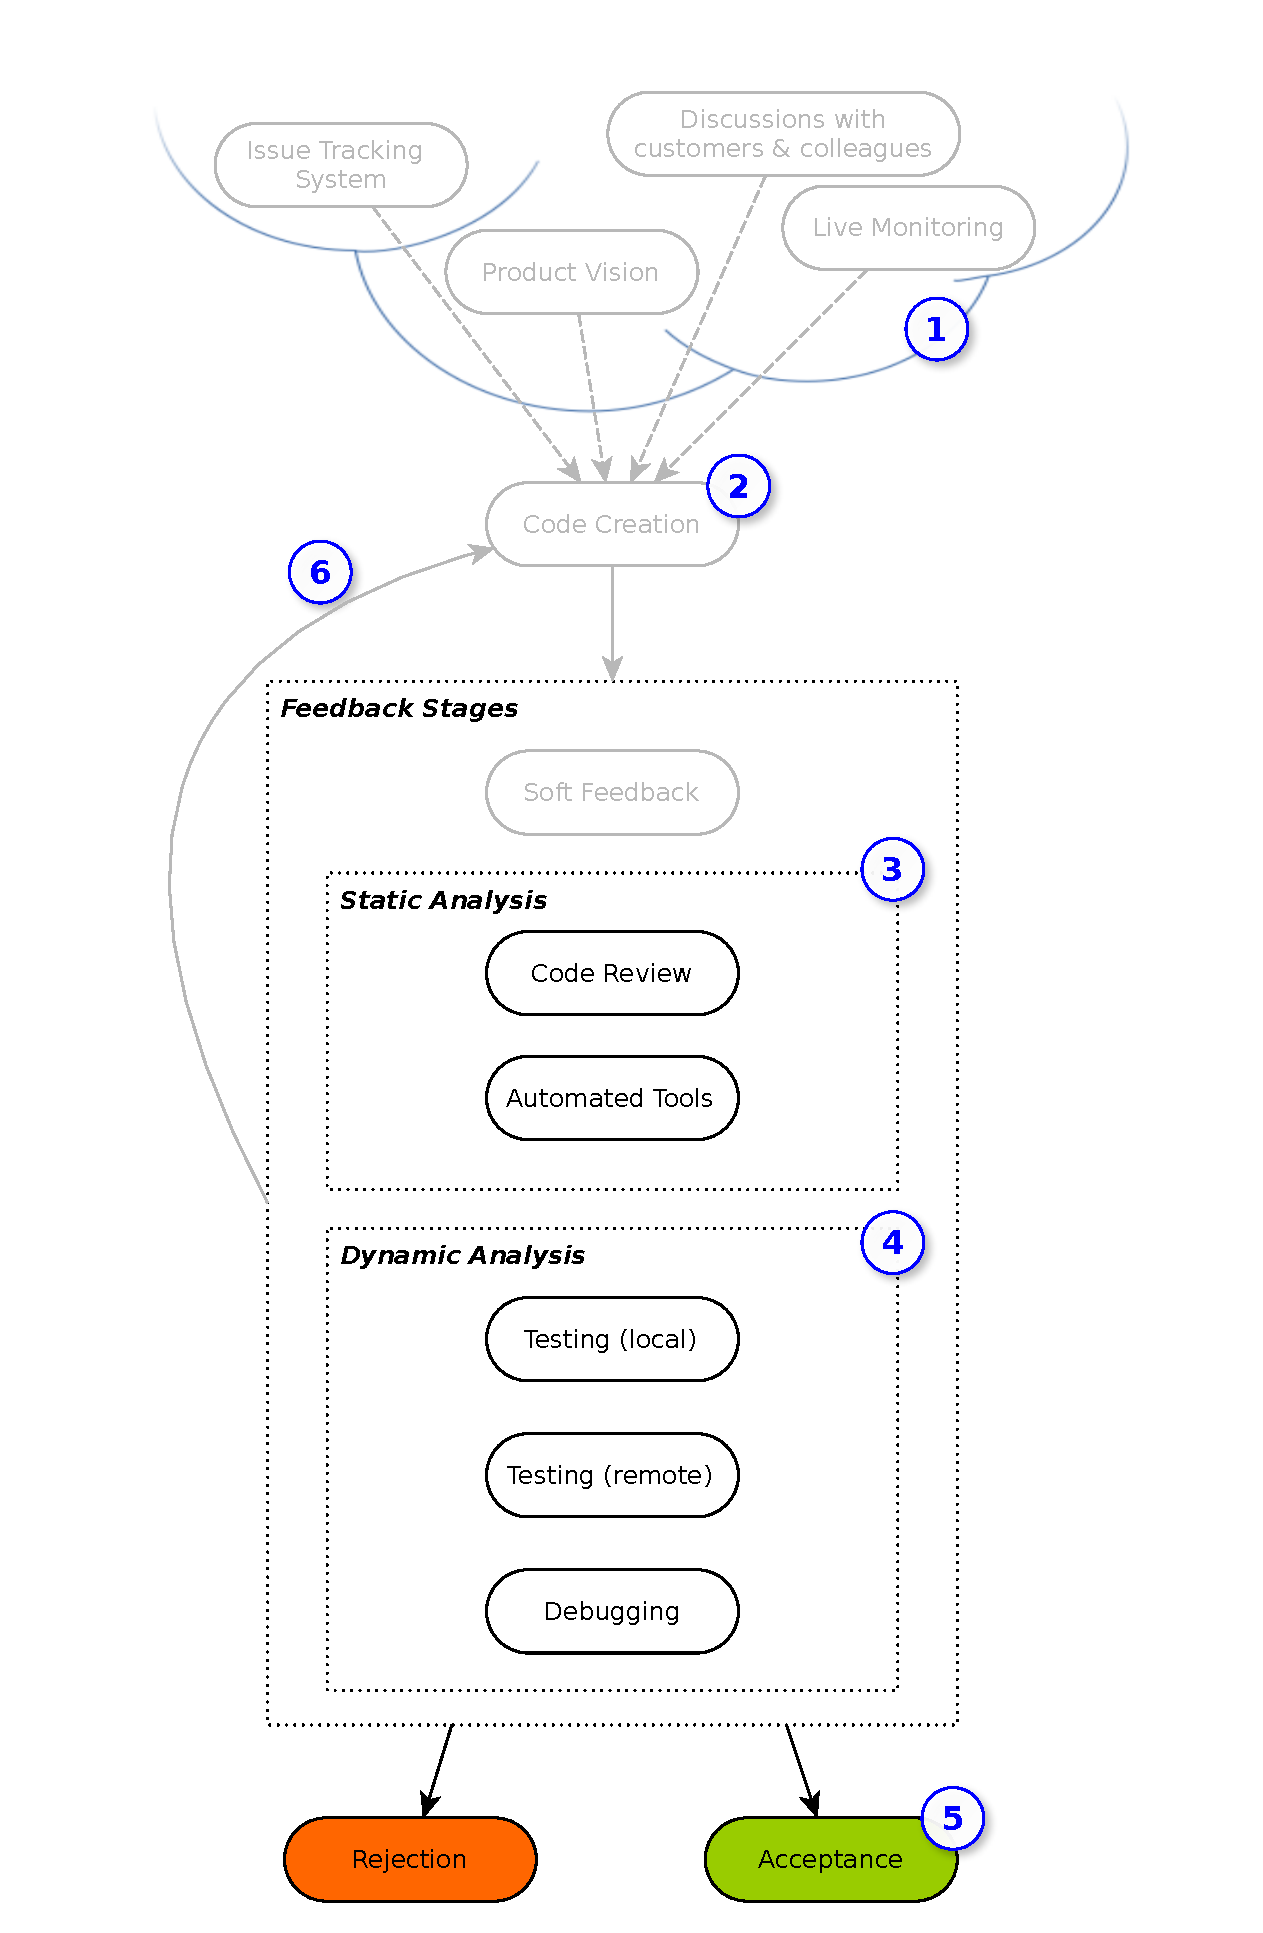
\includegraphics[width=0.65\columnwidth]{development_model_without_papers}
% 	\caption{The stages of the FDD model and their relationship to other
%           Software Engineering concepts.}
% 	\label{fig:devmodel}
% \end{figure}

% We also have lists:

% \begin{enumerate}
%   \item Static Analysis~\circled{3} examines program artifacts or
%     their source code without executing them~\cite{wichmann1995industrial}, while
%  \item Dynamic Analysis~\circled{4} relies on information gathered from their
%   execution~\cite{cornelissen2009systematic}.
% \end{enumerate}

% Or boxes:

% \begin{framed}
% This thesis is concerned with the empirical assessment of the state of the art of how developers
% drive software development with the help of feedback loops.
% \end{framed}

% Or code:
% \begin{lstlisting}[caption={\textsc{TrinityCore}},label={lst:e1}]
%  x += other.x;
%  y += other.y;
%  z += other.y;
% \end{lstlisting}
% \bibliography{Chapter2/chapter2}
% \bibliography{dissertation}
% \printbibliography

% I hope this helps you get started!
% Moritz
